\casesection{Refinement study for channel flow using triangular grids\label{case:channelrefinementtriangles}}


\paragraph*{Purpose}
The purpose of this validation case is to examine the performance of D-Flow FM for the simulation of a schematized uniform and homogeneous channel flow. This validation case focuses on the effects of the refinement of a grid with only triangular cells. The topography comprises a linearly varying bathymetry with a constant slope. 

\paragraph*{Linked claims}
Claims that are related to the current test case are:
\begin{itemize}
\item \clrefnoh{cl:generalGrids}
\end{itemize}


\paragraph*{Approach}
To enable academic comparison of the computational output with a known analytical solution, the topography of the bed varies linearly with a slope $i_b$. Given a discharge $Q$ and a friction coefficient (in this case, Ch\'ezy's factor $C$ is used), an equilibrium water depth $d_e$ can be computed as:
\begin{equation}\label{eq:chezytriangleseqdepth}
d_e = \left(\frac{Q}{B C \sqrt{i_b}}\right)^{2/3}.
\end{equation}
If the grid is refined several times, the order of accuracy of the numerical integration routines can be assessed. For this purpose, only triangular grids are considered (Cartesian grids are considered in case e02-f01-c010).



\paragraph*{Model description}
For this test case, trhee computational grids are generated. The outflow parts of these grids are shown in \Fref{fig:chezytrianglesgrids}. The three grids are of triangular type. The longitudal size $L$ of the domain is 10 km, whereas the lateral size $B$ of the domain is 500 m. 

\begin{figure}[h!]
\begin{center}
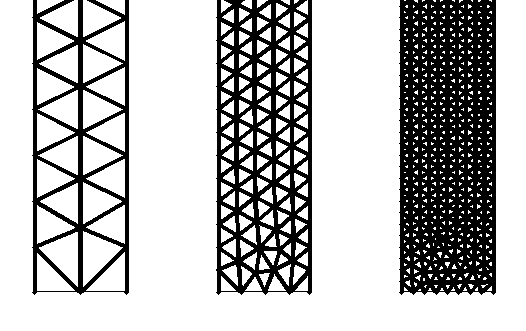
\includegraphics[width=0.5\columnwidth]{figures/grids.png}
\end{center}\caption{From left to right: three triangular grids in order of refinement grade. Each refinement comprises twice as much cells in each direction. Only the outflow part of the grid is shown. \label{fig:chezytrianglesgrids}}
\end{figure}

A discharge $Q$ equal to 2500 m$^3$/s is prescribed. The bottom slope $i_b$ is prescribed to be $10^{-4}$. The bottom level at the inflow boundary is 0 m (w.r.t.\ reference) and at the outflow boundary -1 m (w.r.t.\ reference). The Ch\'ezy friction coefficient $C$ is set to 65 m$^{1/2}$/s. Given the above values, the equilibrium water depth $d_e$ is computed to be 3.89677 m:
\begin{equation}
d_{e} = \left(\frac{Q}{B C \sqrt{i_b}}\right)^{2/3} = \left(\frac{2500}{500 \cdot 65 \cdot \sqrt{10^{-4}}}\right)^{2/3}  = 3.89677\textrm{m}.
\end{equation}
In order to properly impose an outflow boundary that is grid independent, a Neumann-boundary is prescribed at the outflow: $\partial h / \partial x_n = -i_b$, with $h$ the water level. The computational time step is set automatically being restricted by a CFL limit value equal to 0.5. Upstream, the keyword \texttt{jbasqbnddownwindhs} is set to \texttt{1} (relevant for the inflow boundary), whereas \texttt{izbndpos = 0} (relevant for the outflow boundary). For the bed friction, the option \texttt{Conveyance2D = 3} is set (i.e.\ an analytic expression is used for the hydraulic radius).



\paragraph*{Results}
First, recall the quantity \texttt{hu}, which represents the upstream water level (cell center) at the location of a velocity point (cell face). This quantity is used as the water depth within the computation of the bed friction at a velocity point. As a result, the water depth equals the water level at the upstream \emph{cell center} minus the bed level at the \emph{cell face}.

Hence, if a water depth is to be computed as part of the postprocessing, this water depth should be computed in analogy, namely as the difference between the bed level at a velocity point and the upstream water level. This value for \texttt{hu} should then be assessed against the backdrop of the equilibrium depth $d_e$ (see \Eref{eq:chezytriangleseqdepth}) being equal to 3.89677 m, in this case. 

\begin{figure}[h!]
\begin{center}
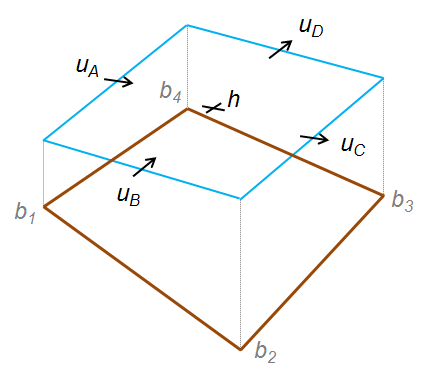
\includegraphics[width=0.5\columnwidth]{figures/computationalcell.png}
\end{center}\caption{Computational cell with surface level $h$, face velocities $u_A$, $u_B$, $u_C$ and $u_D$ and bed levels $b_1$, $b_2$, $b_3$ and $b_4$. \label{fig:chezytrianglescell}}
\end{figure}

The way of postprocessing the water depth can further be clarified by considering an arbitrary computational cell, as shown in \Fref{fig:chezytrianglescell}. Recall that the principal variables are the water level (located at the cell center) and the face-normal velocities (located at the center of the faces). The level of the bed is given in the cell corners. The value of \texttt{hu} at the location of, for instance, velocity $u_C$ is then computed as $h - (b_2 + b_3)/2$ (in case of \texttt{bedlevtyp = 3}; the options \texttt{4} and \texttt{5} take $\min(b_2,b_3)$ and $\max(b_2,b_3)$, respectively, to be subtracted from the water level). However, choosing for \texttt{Conveyance2D = 3} implies an approach according to \texttt{bedlevtyp = 4}.

Since the analytical solution is known for this flow situation, the deviations of the computed results from the analytical results can be measured exactly. As a measure, the $L_2$-norm of the residual $\mathrm{Res}$ (i.e.\ the difference between the analytical and the numerical solution) is taken, defined as
\begin{equation}
\mathrm{Res}_{L_2} = \sqrt{\frac{1}{N} \sum_{i=1}^N \mathrm{Res}_i^2}
\end{equation}
with $N$ the number of evaluated grid locations. Differences with the analytical solution for the five different grids are shown in \Fref{fig:chezytrianglesconvergence} through this measure. 

\begin{figure}[h!]
\begin{center}
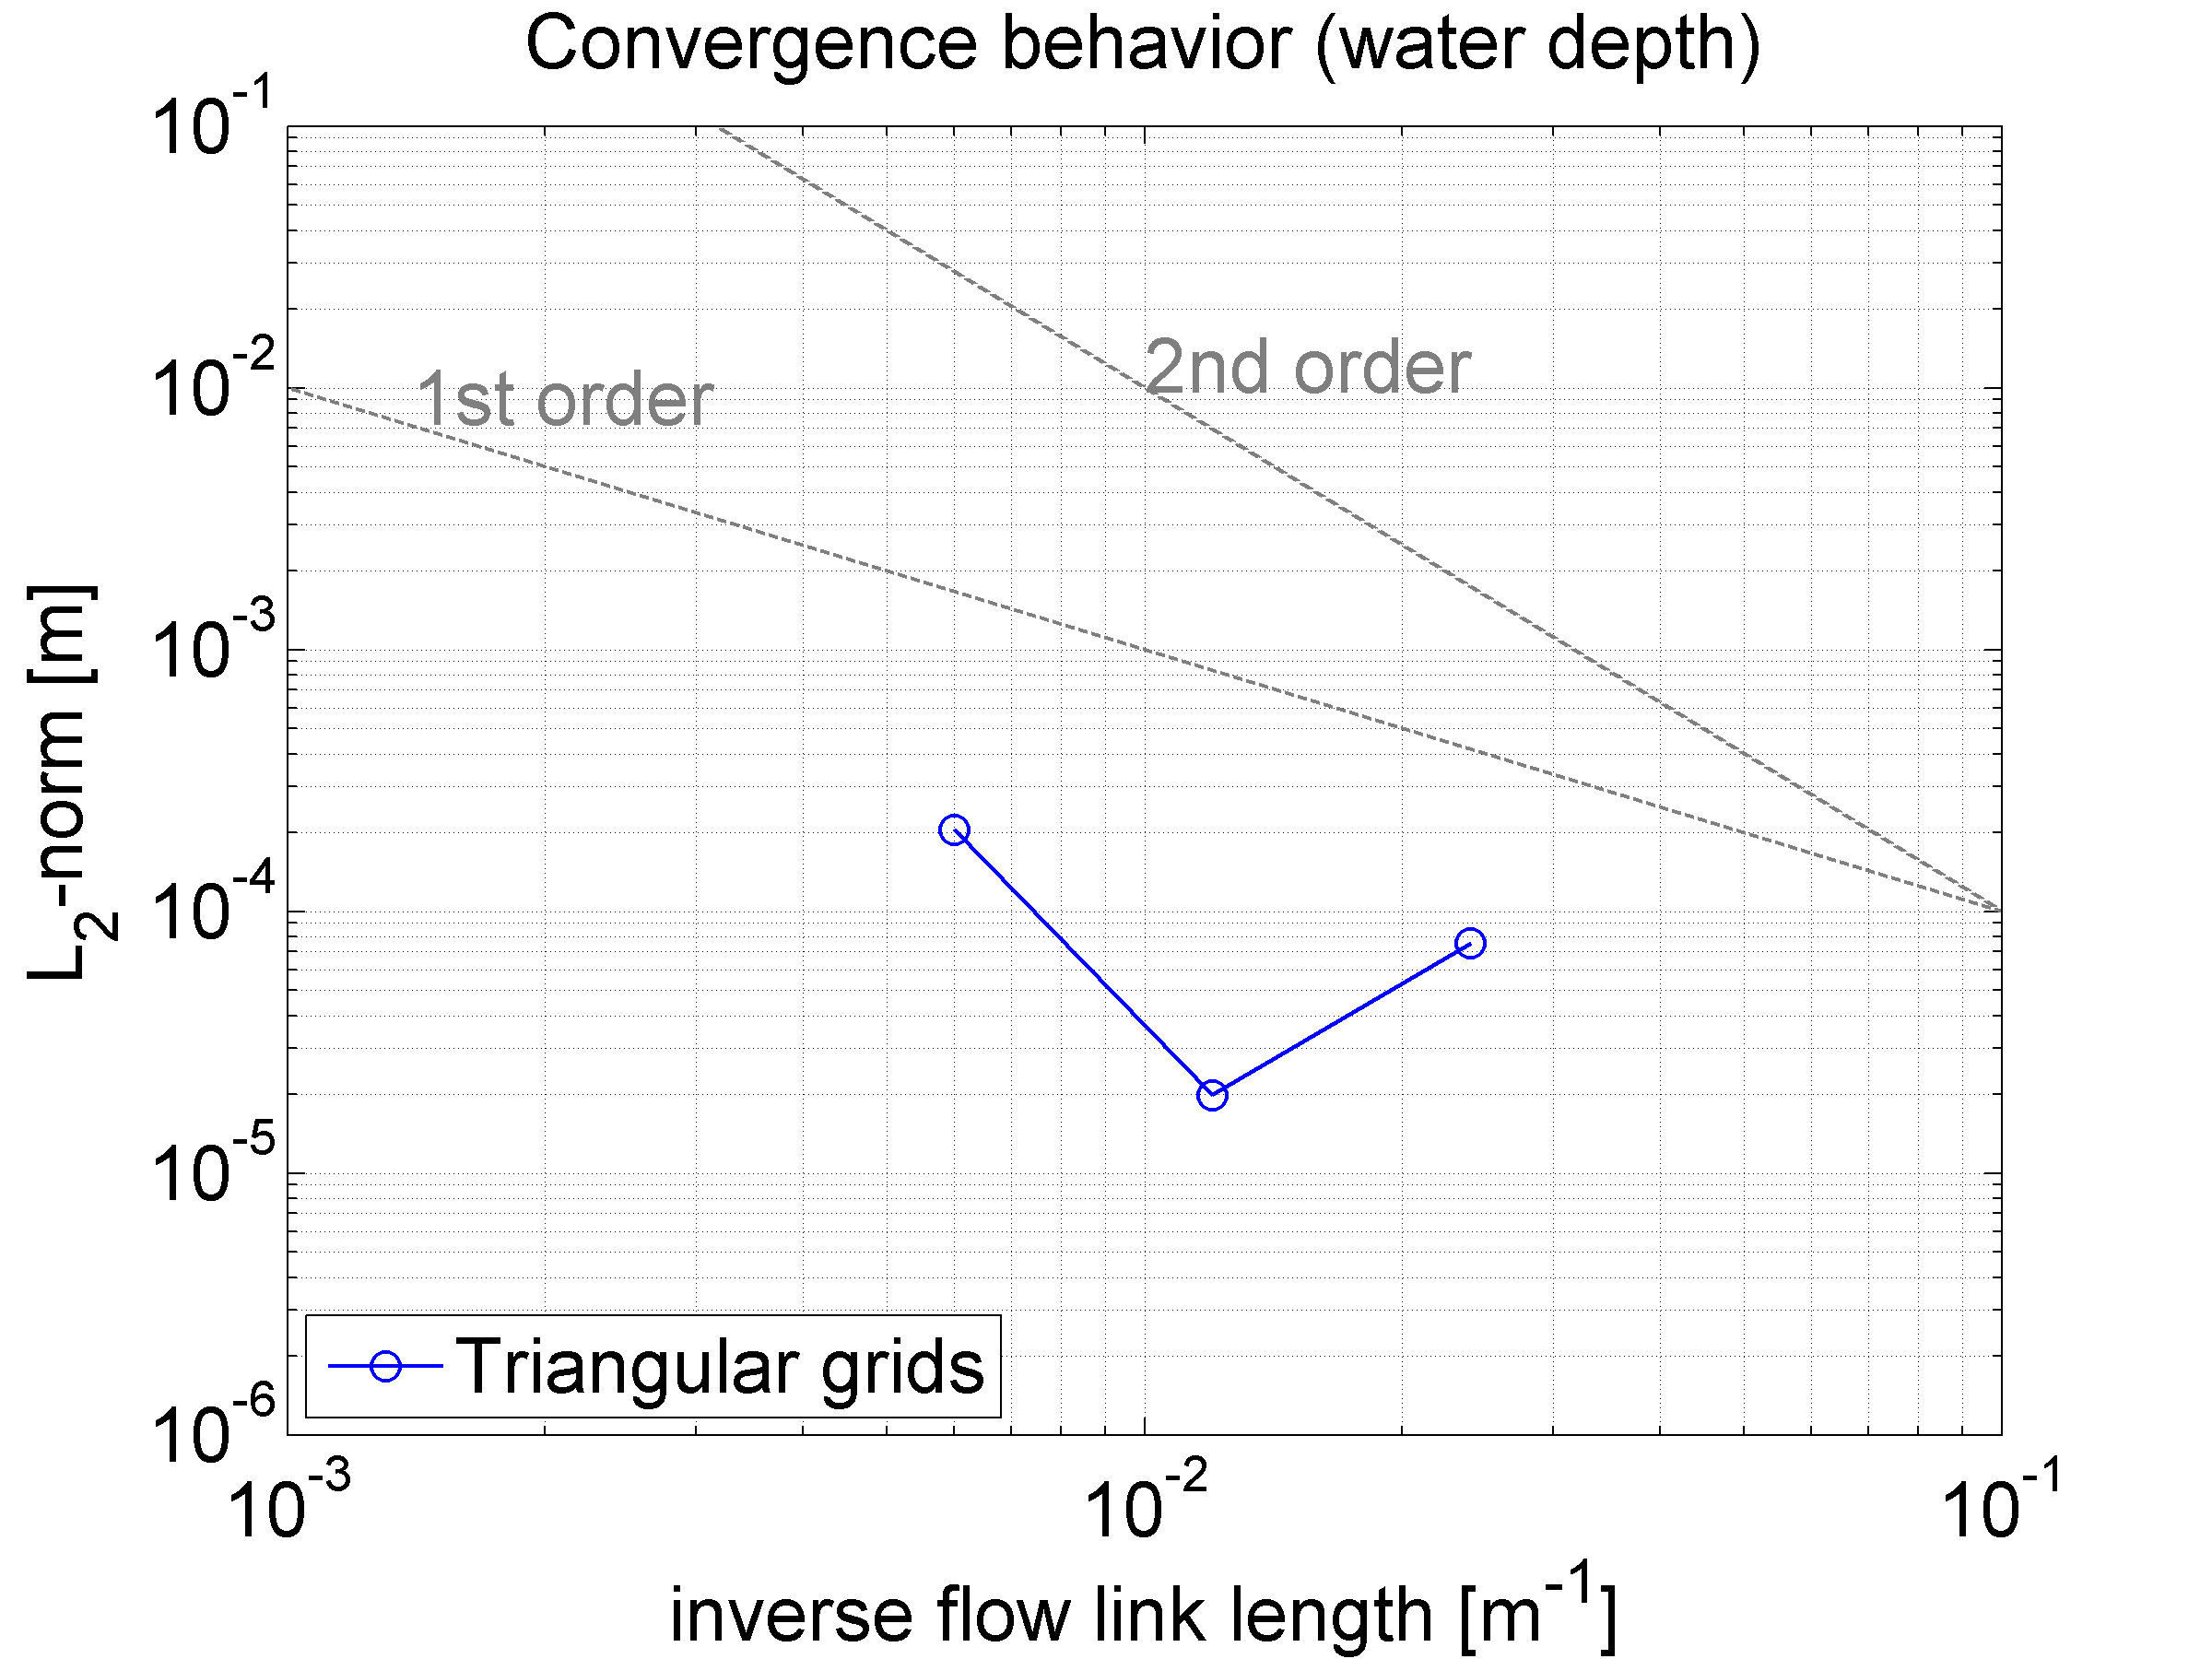
\includegraphics[width=0.48\columnwidth]{figures/hchannelconvergence.png}
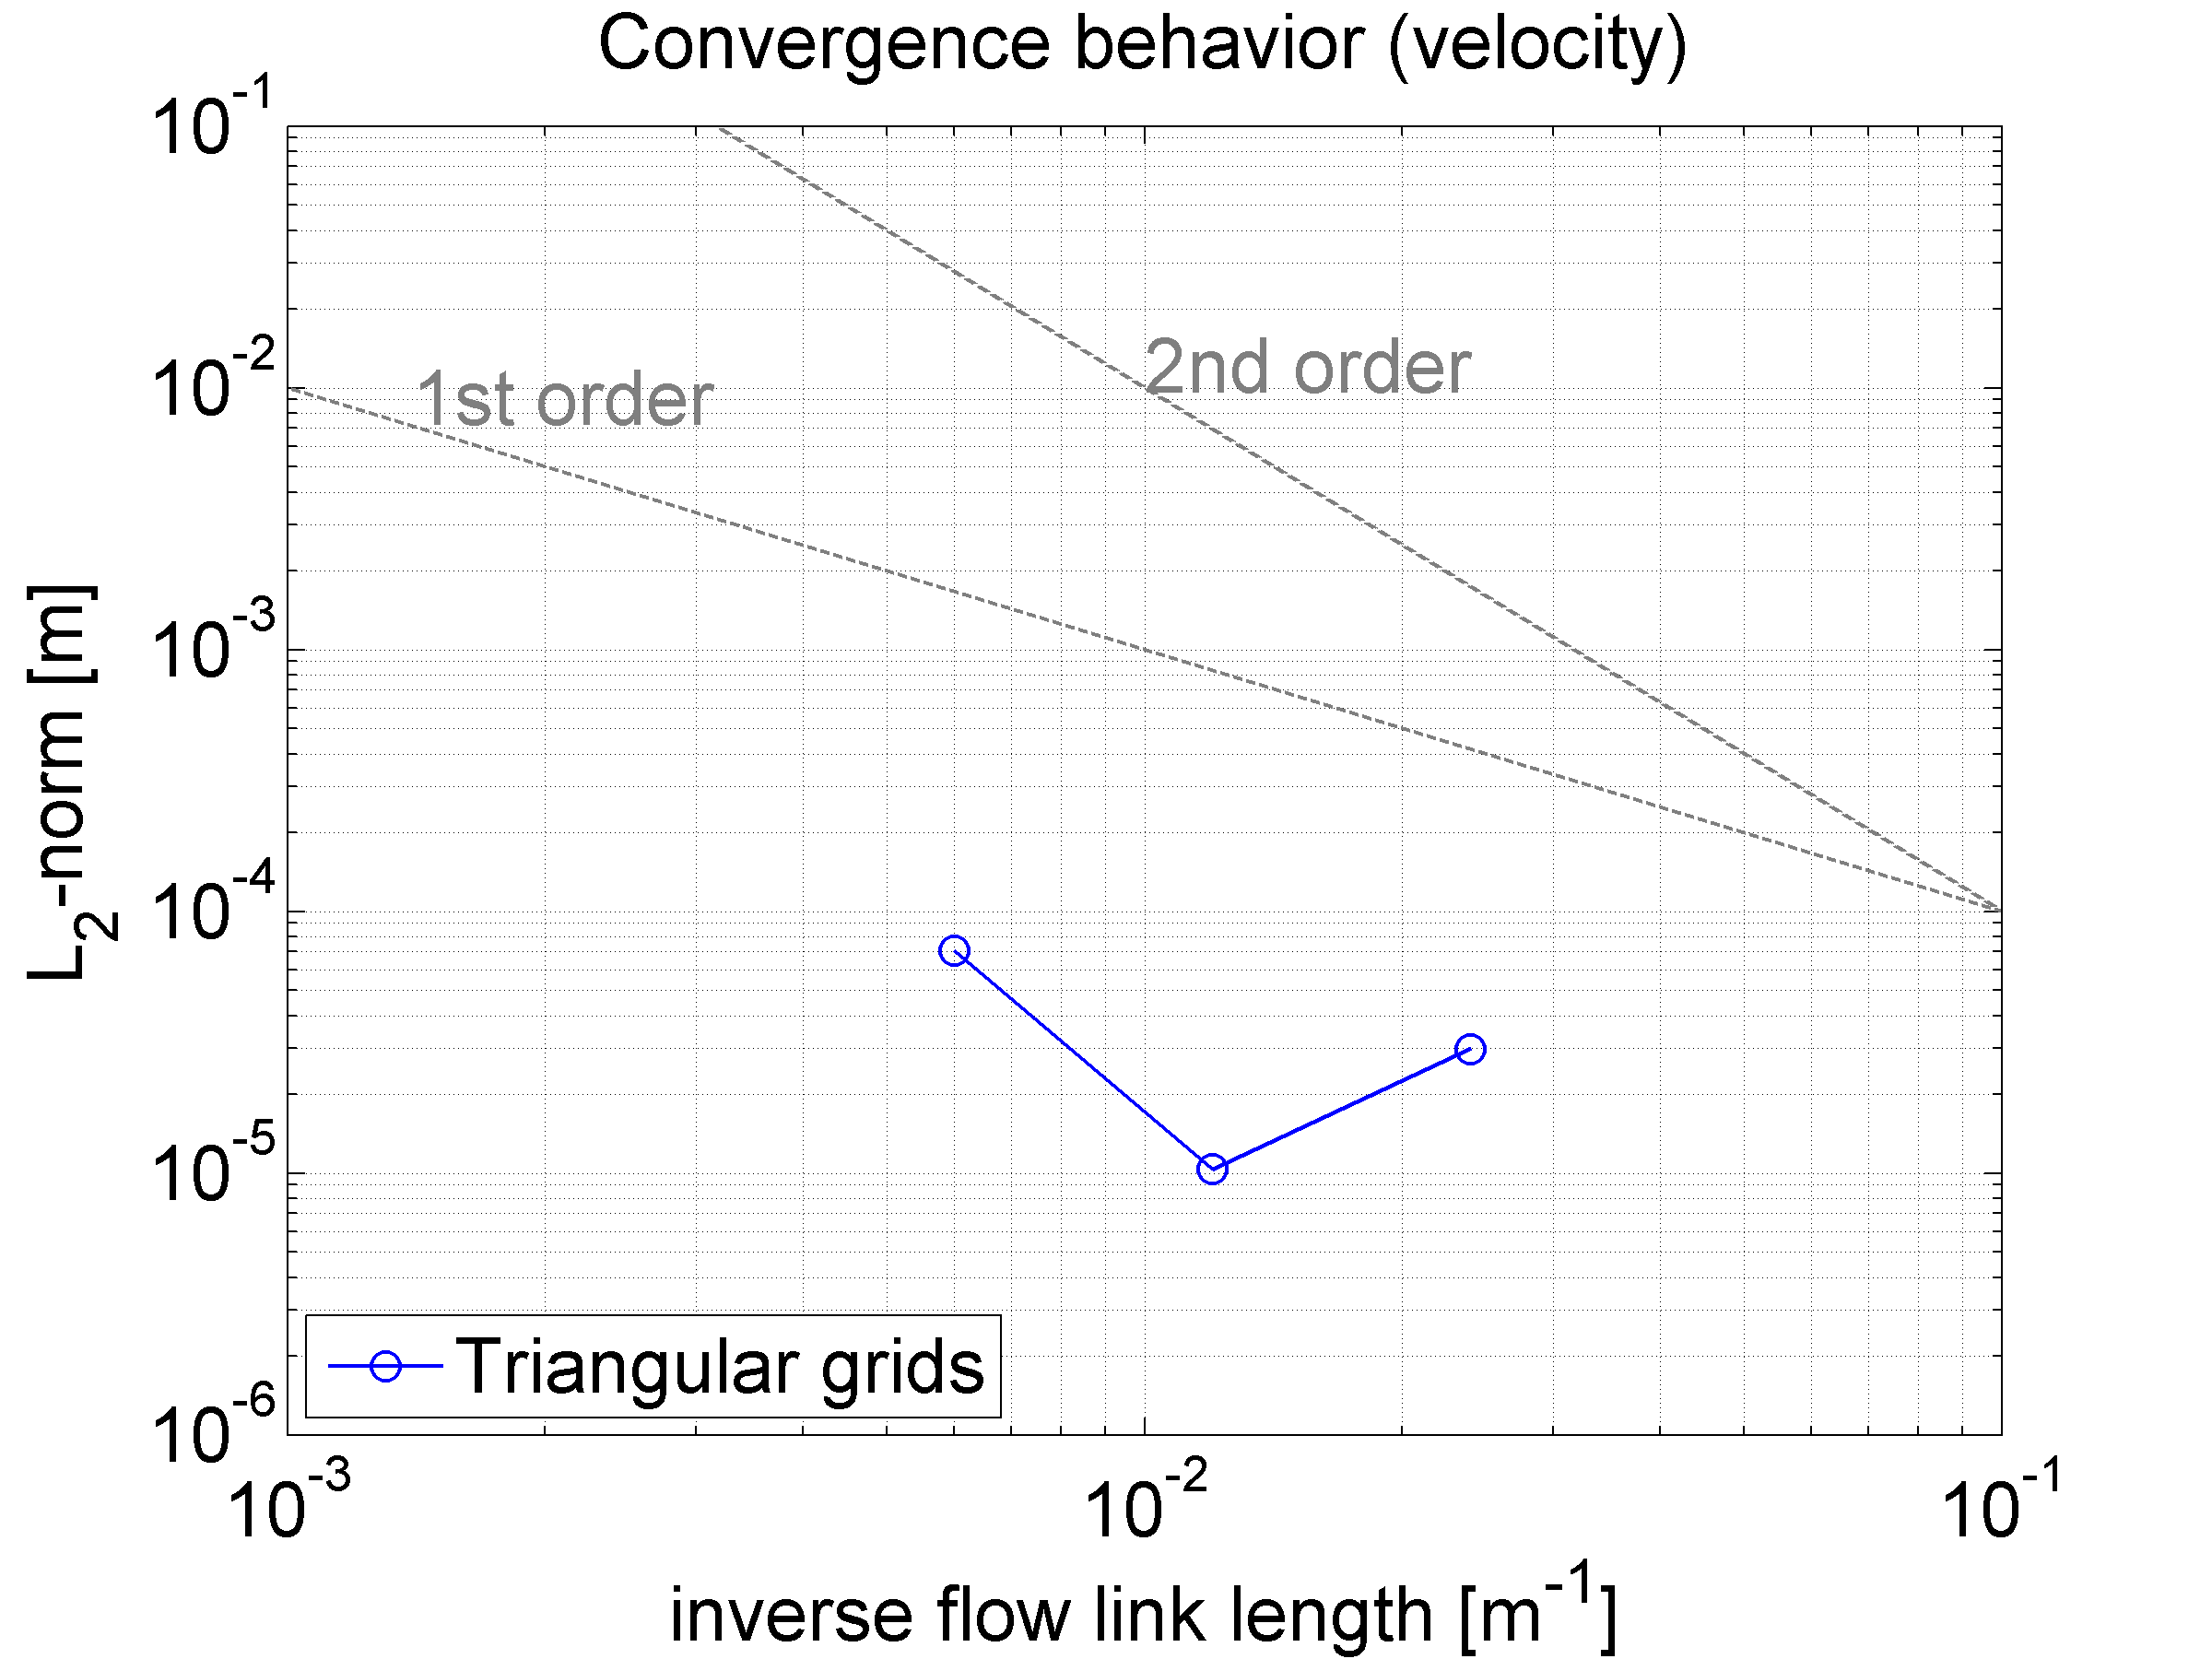
\includegraphics[width=0.48\columnwidth]{figures/uchannelconvergence.png}
\end{center}\caption{Rate of convergence, measured by means of the $L_2$-norm using the analytical solution and the computational output. Left panel: convergence of the computed water depth; right panel: convergence of the computed velocity. \label{fig:chezytrianglesconvergence}}
\end{figure}

\Fref{fig:chezytrianglesconvergence} reveals that the actual differences between the computational and analytical outcomes are significantly larger compared to the ones found for the Cartesian grids (both for the water levels and the velocities, see the documentation for case e02-f01-c010). The residual is assessed with the entire domain taken into account. Morever, the deviations from the analytical solution appear not to converge (both for the water levels and the velocities). The same has appeared to hold for the medium part of the domain, intending to leave potential boundary effects out of consideration. 



\paragraph*{Conclusion}
For the two-dimensional, stationary, homogeneous and uniform channel flow simulations, the following conclusions can be drawn:
\begin{enumerate}
\item on all the three grids (of different grade of refinement), the computational outcomes approximate the analytical outcomes with an accuracy being significantly coarse compared to the simulations on Cartesian grids, both regarding the water levels and the velocities,
\item the differences between the computational and analytical outcomes appear not to converge.
\end{enumerate}



\paragraph*{Version}
This test has been carried out with version dflow-fm-x64-1.1.116.36629.


